%=================================================
\sectionDark{ID3}
%=================================================
\begin{frame}
  \frametitle{TDIDT}
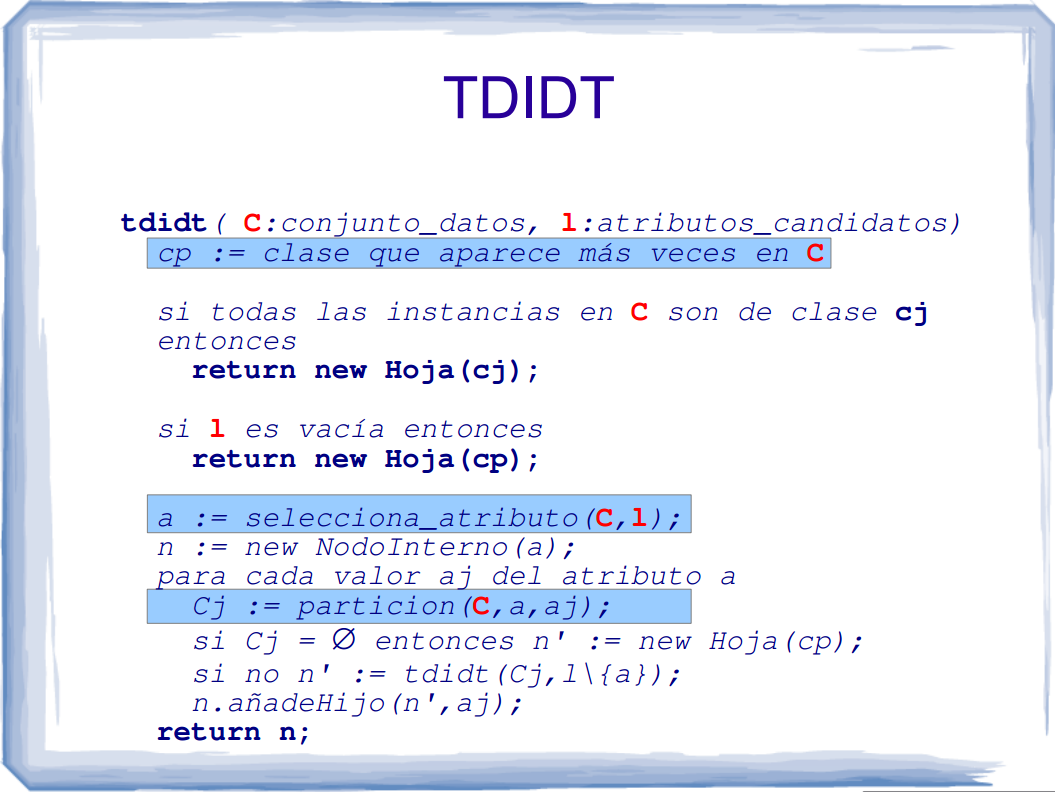
\includegraphics[width=\textwidth]{./images/esquemaTDIDT.png}
\end{frame}

\begin{frame}
  \frametitle{ID3}
\end{frame}

%=================================================
\sectionDark{C4.5}
%=================================================
\begin{frame}
  \frametitle{C4.5}
% Mejoras respecto a ID3
\end{frame}

\begin{frame}
  \frametitle{Algoritmo C4.5}
% Como? implementacion
\end{frame}

\begin{frame}
  \frametitle{Ejemplo}
\end{frame}

\begin{frame}
  \frametitle{Mejoras a C4.5}
\end{frame}

%=================================================
\sectionDark{C5.0}
%=================================================

\begin{frame}
  \frametitle{C5.0}
% Mejoras
\end{frame}


%\begin{frame}
%  \frametitle{Ejemplo}
%\end{frame}

%===== EJEMPLO =====
%\begin{frame}[fragile] % Frame ejemplo 2
%  \frametitle{Ejemplo}
%\end{frame}


